% Journal:
%   Journal of Ambient Intelligence and Smart Environments (JAISE), IOS Press
%   Web Intelligence and Agent Systems: An International Journal (wias)
%   Semantic Web: Interoperability, Usability, Applicability (SW)
% Latex 2e
% Test file iosart2c.tex

%[seceqn,secfloat,secthm,crcready]

% options: wias, jaise, sw
\documentclass{iosart2c}


\usepackage[T1]{fontenc}
\usepackage{times}%

\usepackage{natbib}
%\usepackage[dvips]{hyperref}
\usepackage{amsmath}
\usepackage{dcolumn}
%\usepackage{endnotes}
\usepackage{graphics, url}


\newcolumntype{d}[1]{D{.}{.}{#1}}


\firstpage{1} \lastpage{5} \volume{1} \pubyear{2009}


\begin{document}
\begin{frontmatter}                           % The preamble begins here.

% CHANGE AS SUITED - RL.
%\pretitle{Pretitle}
\title{Enhancing Linguistic Resources with Geospatial Mapping %\thanks{Footnote in title.}
}

\runningtitle{Enhancing Linguistic Resources with Geospatial Mapping}
%\subtitle{Subtitle}

%\review{Name Surname, University, Country}{Name Surname, University, Country}{Name Surname, University, Country}


\author[A]{\fnms{Steven} \snm{Moran}%\thanks{Corresponding author. E-mail: editorial@iospress.nl.}%\thanks{Do not use capitals for the author's surname.}
},
\author[B,C]{\fnms{Richard} \snm{Littauer}}
and
\author[D]{\fnms{Boris} \snm{Villazon-Terrazas}}
\runningauthor{Moran, Littauer and Villazon-Terrazas}
\address[A]{Research Unit Quantitative Language Comparison, Ludwig Maximilian University, Geschwister Scholl Platz 1, D-80539 Munich, Germany\\ 
E-mail: bambooforest@gmail.com} %Steve? Probably not the right email. 


%\address[A]{Journal Production Department, IOS Press, Nieuwe Hemweg 6b, 1013 BG, Amsterdam,\\ The Netherlands\\ E-mail: first@somewhere.com}
%\address[B]{Department first, then University or Company name, Insert a complete correspondence (mailing) address, Abbreviate US states, Include country\\ E-mail: \{second,third\}@somewhere.com}
\address[B]{Department of Intelligent Computer Systems, University of Malta, Msida, MSD2080, Malta}
\address[C]{Computational Linguistics Department, Saarland University, Saarbr\"ucken, 66121, Germany\\  E-mail: littauer@coli.uni-saarland.de}
\address[D]{Intelligent Software Components, iSOCO, S.A., Av. del Partenon 16-18, Madrid, Spain\\
E-mail: bvillazon@isoco.com}

\begin{abstract}
The Linguistics Linked Open Data cloud, created and maintained by the Open Linguistics Working Group, is a (sub-)cloud of the Semantic Web, conforming to the Linked Open Data paradigm. The potential of a very large, interlinking, interoperable ontology for linguistics research is great; however, first adopters may be hesitant to upload their datasets or use the cloud, due to a large learning curve or a lack of obvious uses. Here, we present a research workflow, from a spreadsheet to RDF to visualisation, going through the entire iterative and incremental linked data cycle. We use only freely accessible technologies in the Semantic Web framework, as well as a dataset of lexical and geospatial information of Dogon languages in West Africa. We also present a visualisation of language data from the World Atlas of Language Structures using an endpoint within the LLOD. By doing so, we shed light upon the possibilities of the Semantic Web, and in particular the LLOD, for potential researchers in the digital humanities and computational sciences. %144 words
%The abstract should be clear, descriptive, self-explanatory and no longer than 200 words. It should alsobe suitable for publication in abstracting services. Do not include references or formulae in the abstract.
\end{abstract}

\begin{keyword}
Semantic Web\sep Linked Data\sep LLOD\sep Linguistics\sep Typology\sep Language Resources\sep Geospatial Mapping
%Keyword one\sep keyword two\sep keyword three\sep keyword four\sep keyword five
\end{keyword}

\end{frontmatter}

%http://www.slideshare.net/boricles/linguistic-resources-enhanced-with-geospatial-information

\section{Introduction}
The Semantic Web presents many opportunities for computational linguists and digital humanitarians interested in accessing, presenting, and discovering new information. However, the learning curve for the relevant technologies is steep, and first adopters may be hesitant due to lack of examples of possible uses and ignorance of useful databases for research. The Open Linguistics Working Group (OWLG) \cite{owlg4lrec}, an open community of researchers dedicated towards providing and disseminating openness in the broad field of linguistics, have created and maintain the Linguistics Linked Open Data (LLOD) %Cite something here. 
cloud for that purpose; to make clearly available and freely accessible multiple open databases for use by researchers and commercial companies alike. 

The LLOD is not only freely accessible to researchers, but also openly adaptable for new databases and ontologies. All databases included in the LLOD must subscribe to the Linked Open Data paradigm \citep{bernersLee2006_linkeddata}, which demands that (1) Referred entities should be designated by using URIs,
(2) these URIs should be resolvable over HTTP,
(3) data should be represented by means of specific W3C standards (such as RDF),
(4) and a resource should include links to other resources. These rules facilitate information integration, and thus, interoperability, in that they require that entities can be addressed in a globally unambiguous way, that they can be accessed and interpreted, and that entities that are associated on a conceptual level are also physically associated with each other. 

Furthermore, the following criteria must be met for a new linguistic resource to be included in the LLOD cloud: \begin{enumerate}\item The data is resolvable through HTTP, \item it is provided as RDF, \item it contains links to another data set in the diagram, and \item the entire data set must be available.\end{enumerate}. At the time of writing, the LLOD has {\it draft} status, meaning that several of the resources may point only to resource metadata, although each has been promised to be uploaded and linked to the LLOD in the near future. 

In order to encourage future submission of resources into the LLOD, we present a new resource - a lexical and geospatial database of languages from the Dogon family, in Western Africa. According to the iterative and incremental linked data cycle, all linked data follows a cycle: specification, modelling, generation, publication, and exploitation (which then feeds back into future specification). Here, we go through each of these stages on the way from taking the Dogon spreadsheet to an interactive visualisation using map4rdf. We also present a visualisation using a database already in the LLOD - the World Atlas of Language Structures, WALS \cite{Haspelmath_etal2008}. We hope that these efforts will encourage future researchers to both add to and utilise the LLOD for their own research.  

\section{Related Work}
%I'm note entirely sure of much related work, to be honest. Uhm. Yeah. Boris? Steve?

%% Shouldn't we be describing the Dogon dataset, somewhere?

Regarding language visualisation, there has been some work on displaying language differences on a broad scale. This includes work presenting hierarchical or cross-linguistic data\cite{Rohrdantz:2012, RMB+10}, displaying related languages (gathered from WALS) by geographical proximity and relatedness \cite{LittEACL}, displaying word meaning with a world map \cite{theron}, and displaying language locations on a globe \cite{Haspelmath_etal2008}. However, the authors are not aware of any work using maps derived from data stored in RDF as here, nor of visualisations aimed at displaying language relatedness using lexical items and location together. %Right?

\section{Spreadsheet to geospatial information}
%http://www.slideshare.net/boricles/linguistic-resources-enhanced-with-geospatial-information
In this section we present the specification of the Linked Data Life Cycle presented in \cite{Villazon_2011} as applied to linguistic resources to visualize them with geospatial information.

\subsection{Linguistics Resources}\label{sec:lr}

Our data source consists of a spreadsheet containing GPS coordinates of villages where the different Dogon languages are spoken in Mali. It also contains information about each of these languages, such as the language name, ISO 639-3 language name identifier, the language family and family code, village name, etc. and it can be easily combined via ISO 639-3 codes with dictionary data from each language. These datasets come from the Dogon Languages Project and are freely available online.\footnote{\url{http://dogonlanguages.org}} They were collected by the Dogon Language Project team, mainly Jeffrey Heath, by on-ground reconnaissance or by using language maps; the provenance of each data point is noted in the spreadsheet.\footnote{Steven Moran is affiliated with the Dogon Languages Project and he has worked with the geo spreadsheet data and with the LL-MAP project to bring these data online. See: \url{http://llmap.org/viewer.html?maps=472946}.} Each set of data points per village is associated with a GPS coordinate and can thus be plotted on a world map. Because the set of Dogon languages that belong to the Dogon language family have been until recently poorly documented and described, information about where these languages are spoken in relation to each other can assist linguists in identifying the genealogical relatedness of these languages. The visualization of linguistic information on maps has been a successful method for generating and testing hypotheses (cf.\ \cite{Haspelmath_etal2008}).

%Steve going to need your help here. 

\subsection{Specification}
The process of publishing Linked Data has an iterative incremental life cycle model. Data sources must be identified and analyzed and entities in the data must be assigned a URI. A key element of Linked Data is also the ability to reuse and leverage data that has already been published as Linked Data. By identifying the schema of resources that are to be transformed into Linked Data, conceptual components and their relationships can be properly modeled into the RDF triple format. In the Dogon GPS spreadsheet, we were able to identify fields such as language name, ISO 639-3 code, language family and subfamily, alternative languages spoken in each village, village names, municipality, notes about the speaker's society, and geospatial information and assign them a URI. The spreadsheet also contains information about non-Dogon languages, which allows us to plot the current language contact situation between Dogon and surrounding languages. See Fig.\ \ref{spreadsheet}.

\begin{figure*}[b!hpt]
\caption{Data that contains villages in Mali with language information}\label{spreadsheet}
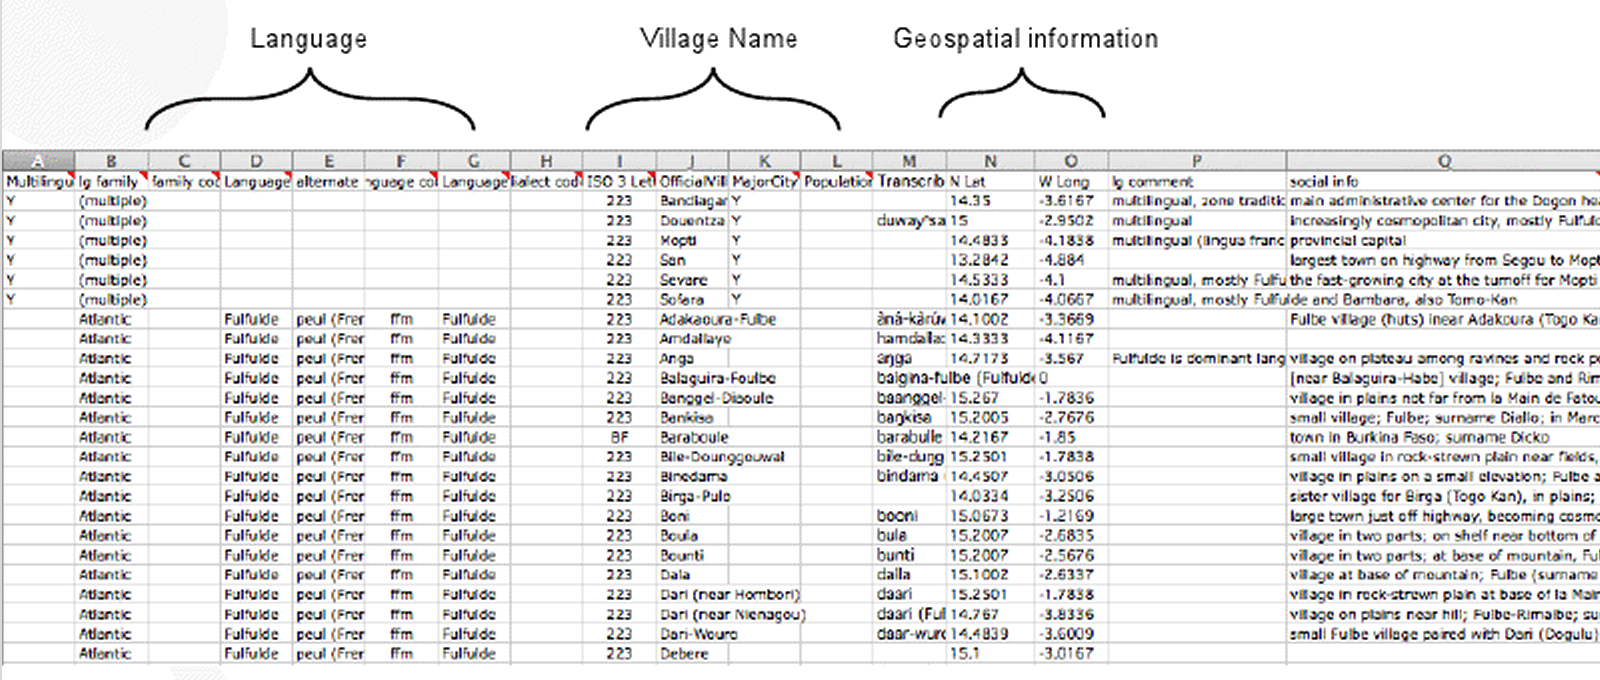
\includegraphics[width=15cm]{img/spreadsheet.png}
\end{figure*}

All resources in the dataset are given dereferenceable URIs and we've attempted to use meaningful names instead of opaque ones. We also reuse URIs where we can, including using the General Ontology of Linguistic Description (GOLD) for morphosyntactic data descriptions \cite{farrar2003linguistic}.\footnote{ \url{http://linguistics-ontology.org/}.} The base URI structure uses the \surl{http://linguistic.linkeddata.es/} namespace. Vocabulary elements are appended with \surl{/ontology/{property|class}} and instances with \surl{/dataset/resource/{r. type|r. name}}. We also reused URIs from the WGS84 Geo Basic Vocabulary for the representation of geospatial data.\footnote{\url{http://www.w3.org/2003/01/geo/}} 

\subsection{RDF Generation}
Next, the spreadsheet data was transformed into RDF. First we imported the spreadsheet into MySQL. Then we defined a set of R2RML mappings. R2RML is a RDF-to-RDF mapping language and we used it to create mappings between elements in the MySQL database table from the spreadsheet and the RDF vocabulary that we defined.\footnote{\url{http://www.w3.org/TR/r2rml/}} Lastly, using the R2RML engine and morph,\footnote{\url{https://github.com/boricles/morph}} we generated the RDF instances using the R2RML defined mappings.

\subsection{Publication}\label{sec:pub}
The RDF data that we generated is stored in a triple store with the Virtuoso software, which we use to publish the data online.\footnote{\url{http://virtuoso.openlinksw.com/}} Integrated with Pubby,\footnote{\url{http://www4.wiwiss.fu-berlin.de/pubby/}} Virtuoso allows us to leverage content management to serve up machine-readable and human consumable webpages that contain information about each village, such as which languages are spoken there, where the village is located, additional information about the society, etc.\footnote{See for example the page on the village Boni: \url{http://linguistic.linkeddata.es/page/mlode/resource/Village/Boni}.} Virtuoso also provides a SPARQL endpoint with which we can query and share the data.

% Virtuoso integrates with Pubby\footnote{\url{http://www4.wiwiss.fu-berlin.de/pubby/}} to publish the results - Pubby is a fronted for endpoints, allowing users to query the data in the Virtuoso server using the SPARQL query language. Once Virtuoso and Pubby are running on data that has been loaded in using the R2RML engine, all of the data is essentially available for humans and computers to read. At this point the data, if it has been specified correctly, if the URIs are HTTP resolvable and if the vocabulary followed set standards, the process of lifting data into the Semantic Web is practically done.  What's left is actually exploiting this data. 

% The generated RDF was then stored in Virtuoso\footnote{\url{http://virtuoso.openlinksw.com/}} open source version. Virtuoso is essentially the server, allowing the RDF data loaded in the Generation step above to be queried using an endpoint. Virtuoso integrates with Pubby\footnote{\url{http://www4.wiwiss.fu-berlin.de/pubby/}} to publish the results - Pubby is a fronted for endpoints, allowing users to query the data in the Virtuoso server using the SPARQL query language. Once Virtuoso and  Pubby are running on data that has been loaded in using the R2RML engine, all of the data is essentially available for humans and computers to read. At this point the data, if it has been specified correctly, if the URIs are HTTP resolvable and if the vocabulary followed set standards, the process of lifting data into the Semantic Web is practically done.  What's left is actually exploiting this data. 

\subsection{Exploitation}
Following the previous steps of specification, RDF generation and publication, we expose the RDF data, enhanced with GPS coordinates, using map4rdf.\footnote{\url{https://github.com/boricles/linked-data-visualization-tools}} map4rdf is a maps viewer of RDF resources with geometrical information built on OpenStreetMap\footnote{\url{http://www.openstreetmap.org/}} and it can be used to visualize information in RDF datasets. Additionally, it is extensible with Google app plugins. The parameters of map4rdf must be set so that the application knows where to locate the endpoint of Dogon data in RDF (that we set up with Virutoso) and which geometry model that we are using (since there different standards for geo-mapping). With the parameters set, a user can open the map4rdf application in his or her web browser and explore the location of villages where Dogon are spoken.\footnote{The map4rdf instantiation for the Dogon villages resides at: \url{http://geo.linkeddata.es/map4rdf-dogon/}.} Fig.\ \ref{fig:map4rdf} provides an illustration.

\begin{figure*}[htb!p]
\centering
%\includegraphics[scale=0.45]{IMGS/detalle_bn.png}
%\includegraphics[width=0.70\textwidth]{IMGS/detalle.pdf}
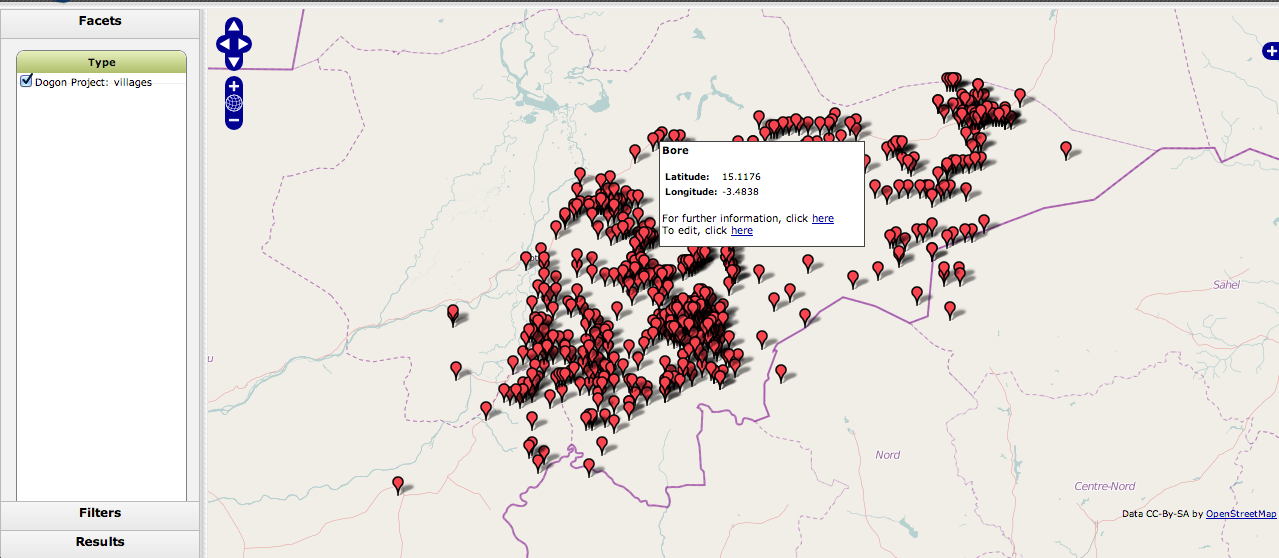
\includegraphics[width=0.99\textwidth]{img/map4rdf.png}
\caption{Visualization of the Dogon villages}
\label{fig:map4rdf}
\end{figure*}

Each point on the map comes from GPS coordinates in the original spreadsheet, which have been transformed into RDF triples and stored in a triple store with Virtuoso. This triple store can be queried with SPARQL or its endpoint can be given as an endpoint for programs like map4rdf to access its data contents.  Each pin in Fig.\ \ref{fig:map4rdf} can be clicked on, showing the village name, its latitude and longitude, and a link for more information about the language. This is shown in Fig.\ \ref{pin.png}.

\begin{figure*}[htb!p]
\centering
%\includegraphics[scale=0.45]{IMGS/detalle_bn.png}
%\includegraphics[width=0.70\textwidth]{IMGS/detalle.pdf}
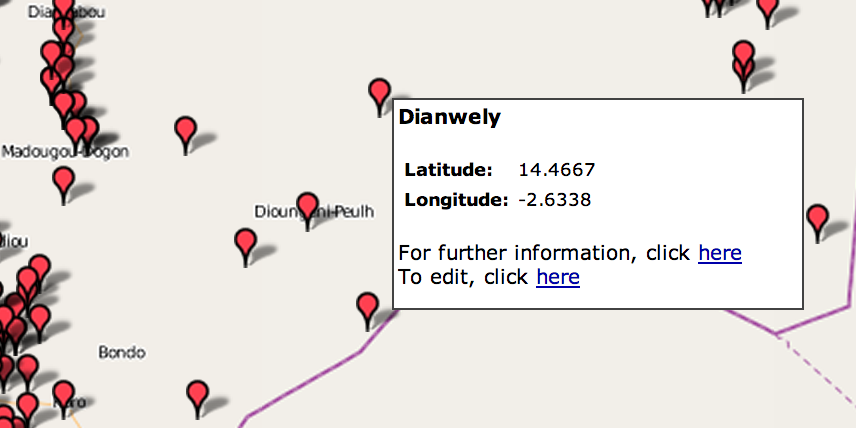
\includegraphics[width=0.99\textwidth]{img/pin.png}
\caption{Clicking on a pin}
\label{pin.png}
\end{figure*}

When clicking on the link for more information, a request is sent to the SPARQL endpoint for all information in the RDF triple store about that particular village. When accessing the data through map4rdf, the endpoint knows through content management to return an HTML page that displays the query results, as shown in Fig.\ \ref{more_information.png}.

\begin{figure*}[htb!p]
\centering
%\includegraphics[scale=0.45]{IMGS/detalle_bn.png}
%\includegraphics[width=0.70\textwidth]{IMGS/detalle.pdf}
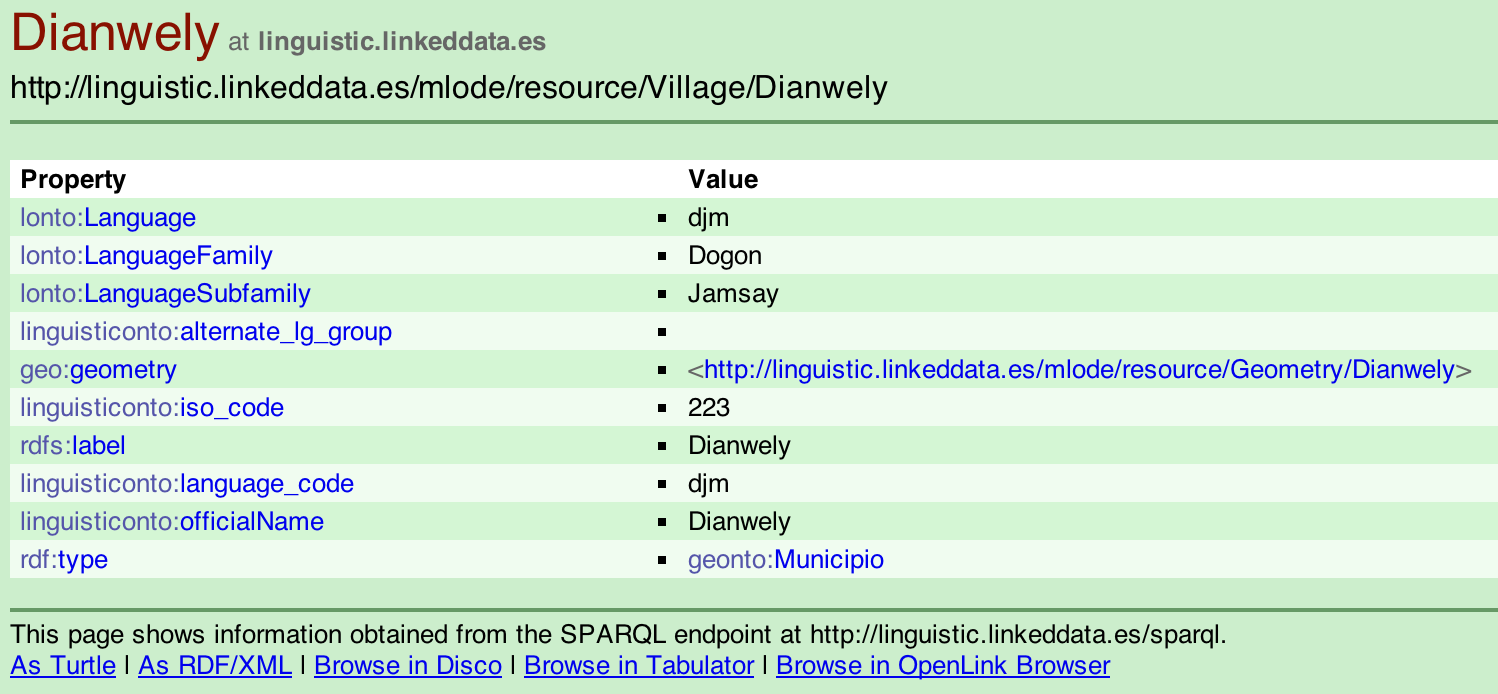
\includegraphics[width=0.99\textwidth]{img/more_information.png}
\caption{More information about a village}
\label{more_information.png}
\end{figure*}



\section{Querying to Geospatial Information}
We also used RDF data gathered automatically from the World Atlas of Language Structures (WALS) \cite{Haspelmath_etal2008}. WALS can be freely accessed from \url{http://wals.info}, and the database can be downloaded as a .csv file. However, there is also an RDF endpoint, which has been integrated with the LLOD cloud. To access the WALS, data, then, we used the SPARQL endpoint available at: \begin{quote}.\url{http://mlode-sparql.nlp2rdf.org/sparql}.\end{quote}

To use the endpoint, go to the link above. Remove the `Default Data Set Name (Graph IRI)' in the top entry box by deleting \url{http://mlode.nlp2rd.org}, so that the box is empty. Write your query into the `Query Text' box, and press `Run Query.' The query will then load. The hyperlink of the loaded query can be used as a way to refer to that result without needing to re-enter the query each iteration. 

%I don't seem to have the query to get the code for each of the languages, and this is kind of repetitious to the other paper. What do you think? Should we include this? 


We plotted this data with map4rdf software. The results of this can be seen here: \url{http://geo.linkeddata.es/map4rdf-wals/#dashboard}

%Boris, you must know the details for this. I don't. 

\section{Conclusions}

We have briefly shown here a workflow to transform data from a simple spreadsheet into an RDF triple store that can queried using a SPARQL endpoint, and an application called map4rdf that uses this endpoint with GPS coordinates to visualize RDF data on a world map. Moreover, the tools that we have used here are open source and freely available. Converting linguistic data into RDF can be a straightforward process and we have shown the steps and some tools to assist in that transformation. There is much data available about languages and their typological features on the Web, which are often available in simple .csv formats. For example, the contents of World Atlas of Language Structures (WALS)\footnote{\url{http://wals.info}} \cite{Haspelmath_etal2008} have been converted from .csv to RDF and are available through the MLODE SPARQL endpoint.\footnote{\url{http://mlode-sparql.nlp2rdf.org/sparql}} It was a trivial task for us to set up map4rdf to point at the WALS RDF data, so that we could also visualize its contents, which contain over 2000 languages' data points. Whereas the online version of WALS already contains maps of typological features of languages, their use is limited and by leveraging RDF as we have with WALS and the Dogon data, we can easily combine these disparate datasets, so that, for example, we can merge data about languages and their typological features from both datasets. This allows us to visualize not only the villages where Dogon languages are spoken, but linguistic features of languages spoken in this area of Mali encoded in WALS. This mashup provides even more detailed information about the features of these different languages, which provides another important data source in untangling the mystery of why Dogon languages are so different than other language families in West Africa. It also shows the power of encoding data in RDF and leveraging RDF tools.


\bibliographystyle{IEEEtran}
\bibliography{bib.bib}

\end{document}

